\documentclass{article}
\usepackage[landscape]{geometry}
\usepackage[utf8]{inputenc}
\usepackage{tikz}
\usetikzlibrary{mindmap,backgrounds}
\pagestyle{empty}
\usepackage[T1]{helvet}
\usepackage[utf8]{inputenc}

\usepackage{tgbonum}

\begin{document}
\pagestyle{empty}



\centering

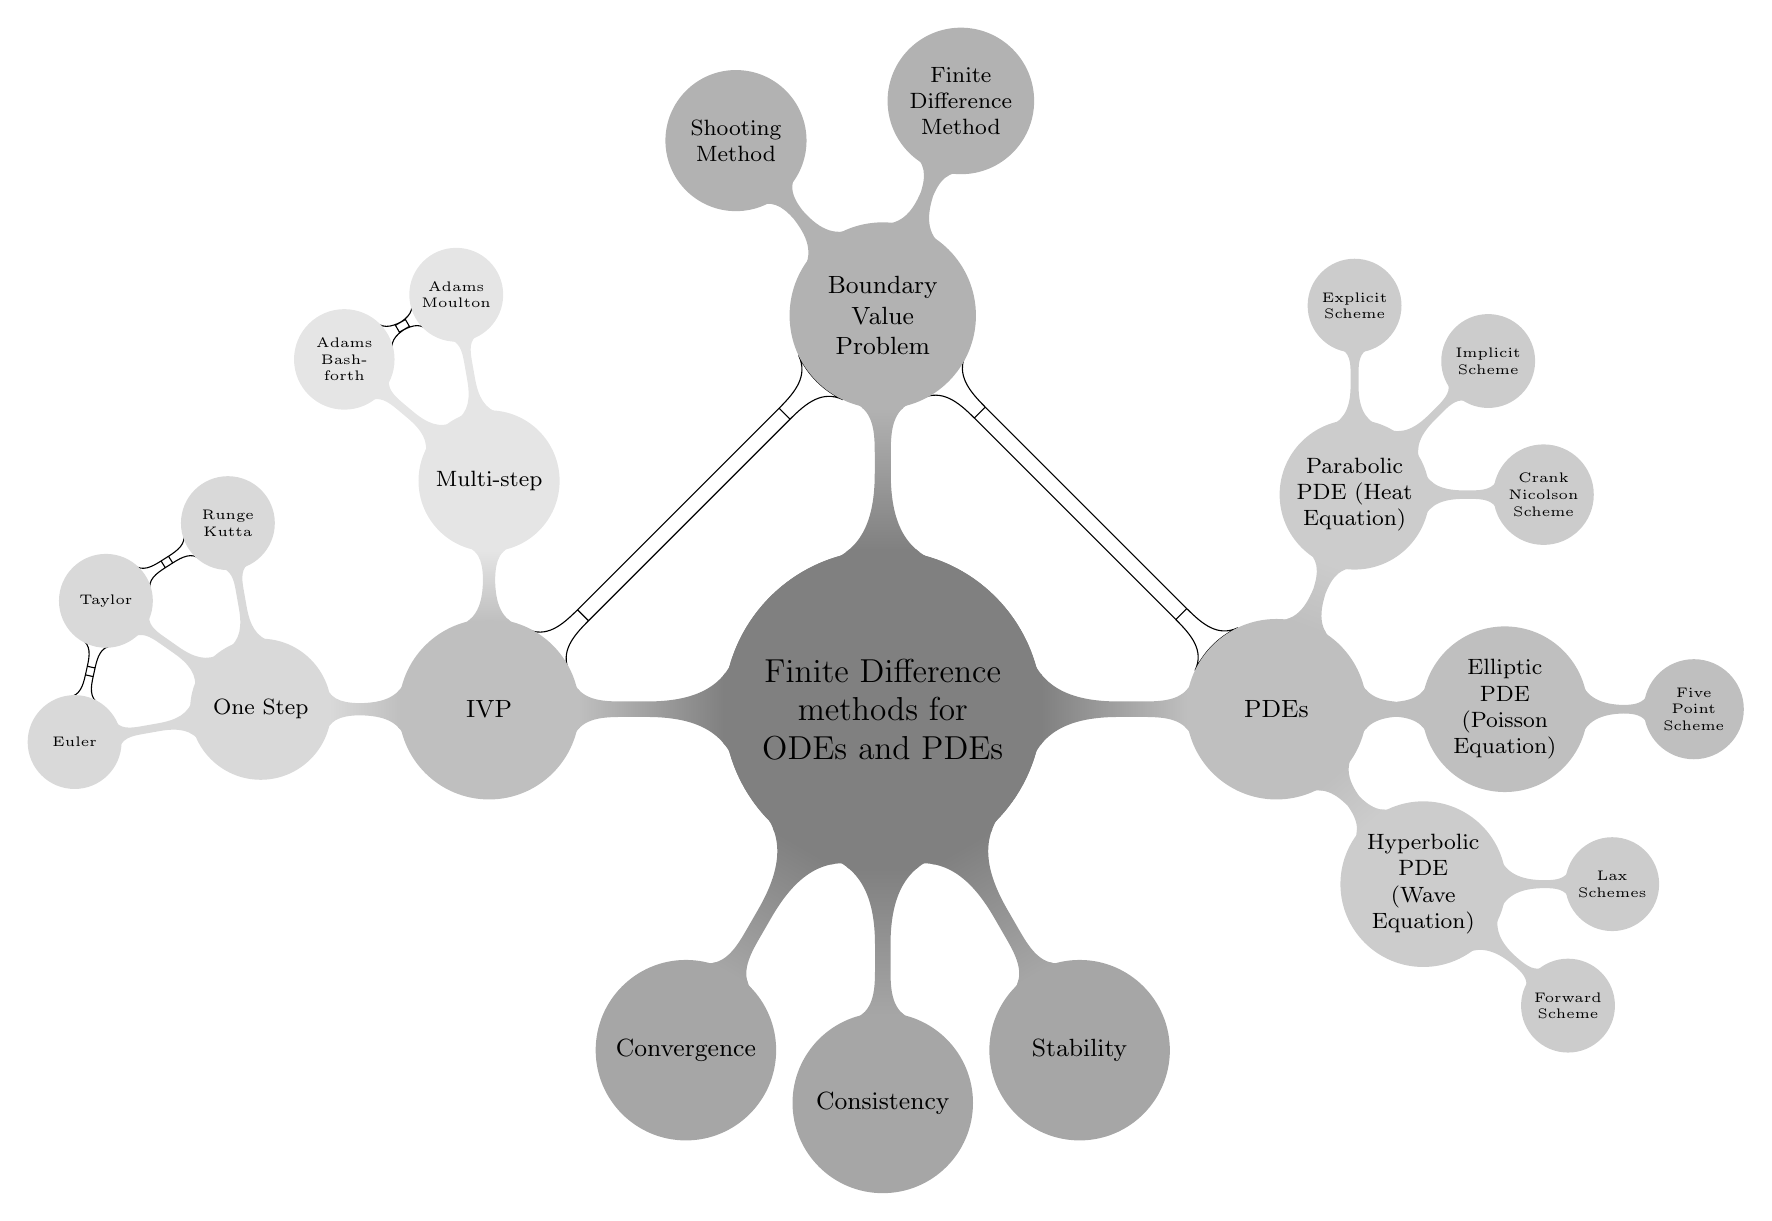
\begin{tikzpicture}




  
  \path[mindmap,concept color=gray,text=black]
    node[concept](na) {Numerical Analysis}
        
        
    child[grow=240, concept color=gray!70] {
      node[concept](convergence) {Convergence}
    }
    child[grow=270,concept color=gray!70] { node[concept](consistency) {Consistency} }
    child[grow=300,concept color=gray!70] { node[concept](ctability) {Stability} 
    }
    % Networks
         child[grow=180,concept color=gray!50]{node[concept] (IVP){ IVP}
    child[grow=90,concept color=gray!20]{node[concept](multi) {Multi-step}
    child [grow=140]
    {node [concept] (bash) {Adams Bashforth}}
    child [grow=100] 
    {node [concept] (moul) {Adams Moulton}}
    }
      % Sorting
      child[grow=180,concept color=gray!30]{node[concept] (sorting){One Step}
    child [grow=190]
    {node [concept] (euler) {Euler}}
    child [grow=145] 
    {node [concept] (taylor) {Taylor}}
    child [grow=100] 
    {node [concept] (runge) {Runge Kutta}
    }}
    }
       child[grow=90,concept color=gray!60]{node[concept] (BVP){Boundary Value Problem}
   child [grow=130]
    {node [concept] (shoot) {Shooting Method}
    }
    child [grow=70]
    {node [concept] (fin) {Finite Difference Method}
    }
   }
     node[concept](pde) {Finite Difference methods for ODEs and PDEs} 
     % Encrypt
     child[grow=0,concept color=gray!50]{node[concept] (PDE){ PDEs}
   child[grow=70,concept color=gray!40]{node[concept] (heat){Parabolic PDE (Heat Equation)}
   child [grow=90]
    {node [concept] (exp) {Explicit Scheme}}
    child [grow=45] 
    {node [concept] (imp) {Implicit Scheme}}
    child [grow=0] 
    {node [concept] (crank) {Crank Nicolson Scheme}}
    }
      % Random Number
 child[grow=0,concept color=gray!50]{node[concept] (poiss){Elliptic PDE (Poisson Equation)}
   child [grow=0]
    {node [concept] (five) {Five Point Scheme}}
   }
   child[grow=-50,concept color=gray!40]{node[concept] (wave){Hyperbolic PDE (Wave Equation)}
   child [grow=-40]
    {node [concept] (five) {Forward Scheme}}
    child [grow=0]
    {node [concept] (five) {Lax Schemes}}
   }
    };

   \begin{pgfonlayer}{background}
    \draw [circle connection bar]
      (euler) edge (taylor)
      (taylor) edge (runge) 
      (bash) edge (moul)
      (IVP) edge (BVP)
      (BVP) edge (PDE) 
      ;
  \end{pgfonlayer}
\end{tikzpicture}\end{document}

\end{tikzpicture}
\end{document}